\documentclass[10pt]{article}
\usepackage[utf8]{inputenc}
\usepackage[T1]{fontenc}
\usepackage[version=4]{mhchem}
\usepackage{stmaryrd}
\usepackage[margin=0.5in, tmargin=1in]{geometry}
\usepackage{xcolor}
\usepackage{graphicx}
\usepackage{multicol}

\usepackage{fancyhdr}
\pagestyle{fancy}
\fancyhf{}
\fancyhead[L]{Math 1A Spring 2024 Notes}
\fancyhead[R]{Alexis Fernandez}
\renewcommand{\headrulewidth}{0.4pt}

\usepackage{enumitem}
\setlist[enumerate]{leftmargin=*}

\usepackage{amsmath, amsfonts, amssymb}

\author{}
\date{}


\begin{document}

\section*{\centering Note 16 - Derivatives and the Shape of the Graph}

\subsection*{Maximum and Minimum Values}

\begin{itemize}
    \item A graph can be described with its minimums and maximums, defined as follows:
    \begin{itemize}[label=$\circ$]
        \item $f(c)$ is the \textbf{absolute maximum value} of $f$ on $D$ if $f(c) \geq f(x)$ for all $x \in D$.
        \item $f(c)$ is the \textbf{absolute minimum value} of $f$ on $D$ if $f(c) \leq f(x)$ for all $x \in D$. \\
        \textit{Note: $c$ is a number in the domain $D$ of a function $f$}.
        \item $f(c)$ is a \textbf{local maximum value} of $f$ if $f(c) \geq f(x)$ when $x$ is \textit{near} $c$.
        \item $f(c)$ is a \textbf{local minimum value} of $f$ if $f(c) \leq f(x)$ when $x$ is \textit{near} $c$. \\
        \textit{Note: \textbf{Near} meaning true on some interval containing $c$.}
    \end{itemize}

    \item These definitions lead to the following properties and theorems:
    \begin{itemize}[label=$\circ$]
        \item A local min/max \textit{cannot} be an endpoint of the domain.
        \item An absolute min/max is \textit{either} a local min/max \textit {or} an endpoint.
        \item \textbf{The Extreme Value Theorem}: \\ If $f$ is continuous on a closed interval $[a,b]$, then $f$ attains an absolute maximum value, $f(c)$, and an absolute minimum value, $f(d)$, at some numbers $c, d \in [a,b]$.
        \item \textbf{Fermat's Theorem}: If $f$ has a local maximum or minimum at $c$, and if $f'(c)$ exists, then $f'(c) = 0$.
    \end{itemize}
    
    \item \textbf{Critical number}: A number $c$ in the domain of $f$ such that either $f'(c)=0$ or $f'(c)$ does not exist. \\
    {\color{blue}
    \textbf{Example:}} Find the critical number of $f(x)=x^{3/5}(4-x)$ \\
    {\color{magenta}
    \textbf{Procedure:} Find the derivative, $f'(x)$. Then, set $f'(x) = 0$ and find the values of x where $f'(x)$ does not exist.}
    \begin{align*}
        f'(x) &= x^{3/5}(-1)+\frac{3}{5}x^{-2/5}(4-x) & \qquad \text{\color{magenta}{Use the product rule to derive the function.}}\\
        &= -x^{3/5}+\dfrac{3(4-x)}{5x^{2/5}} & \qquad \text{\color{magenta}{Simplify.}}\\
        &= \dfrac{-5x+3(4-x)}{5x^{2/5}} & \qquad \text{\color{magenta}{Multiply the first term by $\frac{5x^{2/5}}{5x^{2/5}}$ to have a common denominator.}}\\ 
            &= \dfrac{-8x+12}{5x^{2/5}} & \qquad \text{\color{magenta}{Simplify the numerator.}}\\
    \end{align*}
    {\color{magenta}
    Now that we have $f'(x)$, check the two cases for critical numbers: }
    \begin{multicols}{2}
        \begin{itemize}[label=$\circ$]
            \item Case 1: $f'(c) = 0$
            \begin{flalign*}   
            \dfrac{-8x+12}{5x^{2/5}} &= 0 &\\
            -8x + 12 &= 0 \implies x = \frac{3}{2} &
            \end{flalign*}

            \item Case 2: $f'(c)$ DNE \\
            \textit{Recall: A rational function is undefined when the \break denominator is 0.}
            \begin{flalign*}   
            5x^{2/5} &= 0 \implies x = 0 &
            \end{flalign*}

        \end{itemize}
    \end{multicols}

    \item If $f$ has a local maximum or minimum at $c$, then $c$ is a critical number of $f$.
\end{itemize}

\newpage

\subsection*{The Closed Interval Method}

To find the absolute minimum and maximum values of a continuous function $f$ on a closed interval $[a, b]$, use the \textbf{Closed Interval Method}. \\

\noindent
{\color{magenta}
\textbf{Procedure:}
\begin{enumerate}
        \item {\color{black}Find the values of $f$ at the critical numbers  of $f$ in $[a,b]$.}
    \item {\color{black} Find the values of $f$ at the endpoints of the intervals.}
    \item {\color{black} The largest of  the values from steps (1) and (2) is the absolute maximum. The smallest is the absolute minimum.} \\
\end{enumerate}}

\noindent 
{\color{blue}
\textbf{Example:}} Find the absolute minimum and maximum of $f(x)=x^3-3x^2+1$ on the interval $[-\frac{1}{2}, 4]$. \\

{\color{magenta}
\textbf{Step 1:} Find the critical numbers of $f$:}
\begin{align*}
    f'(x) &= 3x^2-6x & \qquad \text{\color{magenta}{Use the power rule to derive the function.}}\\
    &= 3x(x-2) & \qquad \text{\color{magenta}{Factor to solve for $x$.}}\\
    \implies x &= 0, 2 & \qquad \text{\color{magenta}{$f$ has critical numbers at $x=0$ and $x=2$.}}\\
\end{align*}

{\color{magenta}
And evaluate $f$ at the critical numbers:} \\
{\color{red}\indent \textit{Note: Make sure to plug critical numbers into the original $f(x)$, not the $f'(x)$ you calculated above!}}
\begin{multicols}{2}
    \begin{itemize}[label=$\circ$]
        \item At $x=0$:
        \begin{flalign*}   
        f(0) &= (0)^3-3(0)^2+1 &\\
        &= 0 - 0+1 &\\
        &= 1
        \end{flalign*}

        \item At $x=2$:
        \begin{flalign*}   
        f(2) &= (2)^3-3(2)^2+1 &\\
        &= 8 - 12 + 1 &\\
         &= -3
        \end{flalign*}

    \end{itemize}
\end{multicols}

{\color{magenta}
\textbf{Step 2:}
The values of $f$ at its endpoints are:}
\begin{multicols}{2}
    \begin{itemize}[label=$\circ$]
        \item At $x=-\frac{1}{2}$:
        \begin{flalign*}   
        f(-\frac{1}{2}) &= (-\frac{1}{2})^3-3(-\frac{1}{2})^2+1 &\\
        &= -\frac{1}{8} - \frac{3}{4}+1 &\\
        &= \frac{1}{8}
        \end{flalign*}

        \item At $x=4$:
        \begin{flalign*}   
        f(4) &= (4)^3-3(4)^2+1 &\\
        &= 64 - 48 + 1 &\\
         &= 17
        \end{flalign*}

    \end{itemize}
\end{multicols}

\begin{quote}
{\color{magenta}
\textbf{Step 3:}
Comparing all these values:}
    \begin{itemize}[label=$\circ$]
        \item The absolute minimum of $f$ is $-3$ attained at $x=2$.
        \item The absolute maximum of $f$ is $17$ attained at $x=4$.
    \end{itemize}
\end{quote}

\newpage

\subsection*{The Mean Value Theorem}

To understand the Mean Value Theorem, we must first understand Rolle's Theorem:

\begin{itemize}
    \item \textbf{Rolle's Theorem}: \\
    If $f$ is a function that satisfies:
        \begin{itemize}[label=$\circ$]
            \item $f$ is continuous on the closed interval $[a,b]$.
            \item $f$ is differentiable on the open interval $(a, b)$  -- everywhere except the endpoints.
            \item $f(a)=f(b)$
        \end{itemize}
    Then, there is a number $c \in (a,b)$ such that $f'(c) = 0$.
\end{itemize}

Some examples:
\begin{figure}[h]
        \centering
        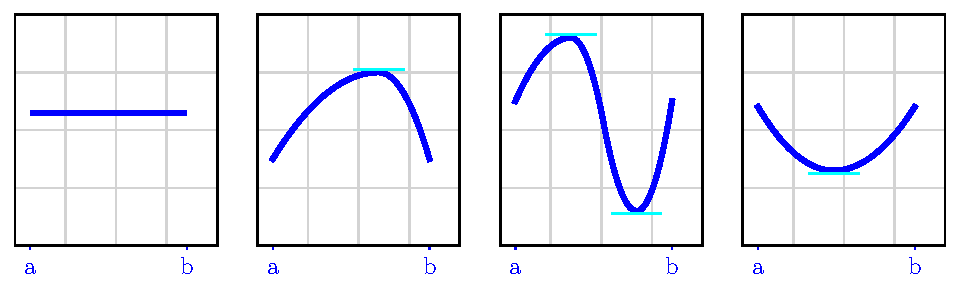
\includegraphics{images/note16/rolles.pdf}
    \end{figure} 

\begin{itemize}
    \item \textbf{Mean Value Theorem}: \\
    If $f$ is a function that satisfies:
        \begin{itemize}[label=$\circ$]
            \item $f$ is continuous on the closed interval $[a,b]$.
            \item $f$ is differentiable on the open interval $(a, b)$.
        \end{itemize}
    Then, there is a number $c \in (a,b)$ such that $$f'(c) = \frac{f(b)-f(a)}{b-a}$$
    or, $f(b)-f(a)=f'(c)(b-a)$.

    \item At some point, the average rate of change = instantaneous rate
    \
\end{itemize}

\end{document}

